%!TeX spellcheck = en-US
\documentclass{article}
\usepackage{bookmark}
\usepackage{color}
\usepackage{amsmath}
\usepackage{hyperref}
\usepackage{listings}
\usepackage{xcolor}
\usepackage{indentfirst}
\usepackage{graphicx}
\usepackage{amsfonts}
\usepackage{hyperref}
\usepackage[top=2cm, bottom=2cm, left=2cm, right=2cm]{geometry}  
\usepackage{algorithm}  
\usepackage{algorithmicx}  
\usepackage{algpseudocode} 
\usepackage{forest}
\newcommand{\bigO}{\mathcal{O}}

 
\renewcommand{\algorithmicrequire}{\textbf{Input:}}  
\renewcommand{\algorithmicensure}{\textbf{Output:}}  

\begin{document}
\noindent

%========================================================================
\noindent\framebox[\linewidth]{\shortstack[c]{
\Large{\textbf{VE 477 Homework 3}}\vspace{1mm}\\
Wang Yichao, ID: 517370910011}}

\begin{itemize}

\item \textbf{Exercise 1.}
1. Similar to BFS, DFS is used for search problems. DFS has the priority of depth and requires less space complexity compared to BFS. 

2. Topology sorting is used for directed acyclic graph(DAG). if $A\to B$, then A is sorted before B.

3. Hamiltonian path is NP. 

\begin{algorithm}[H]  
    \caption{Hamilton}  
    \begin{algorithmic}[1]  
        \Require a graph $G(V, E)$ which is DAG
        \Ensure whether contains a Hamilton path
        \Comment{first topology sort then judge}
        \Function {topology} {$G(V, E)$}
        	\State L = $\{\}$
        	\State S = nodes without incoming edge
        	\While{S is not empty}
        		\State choose a node n from S
        		\State remove n from S
        		\State $L = L \cup \{n\}$
        		\For {node m with edge e = $n\to m$ }
        			\State remove e from E
        			\If {m has no incoming edge}
        				\State $S = S \cup \{m\}$
        			\EndIf
        		\EndFor
        	\EndWhile
        	\State \Return L
        \EndFunction
        \State $L = topology(G(V, E))$
        \For{$i = 0:|L|:1$} 
        	\If {$L[i]\to L[i+1] \in E$}
       			\State Continue
       		\Else
        		\State \Return False
        	\EndIf
        \EndFor

        \Return True
            
    \end{algorithmic}  
\end{algorithm}

4. it is obvious that line 17 to line 23 has complexity of $\bigO (|V|)$.

for topology sort, we notice that the while loop has $\bigO (|V| + |E|)$, the remove of edge means that we has $\bigO (|E|)$. We should be careful about the insert m to S step, otherwise the while loop has only $\bigO (|V|)$. In all, the time complexity is $\bigO (|V| + |E|)$.

5. The decision problem in this question is only in P. But the Hamilton path problem is NP-complete.

\item \textbf{Exercise 2.}

1. no, using stirling's formula, $n ! \sim  n^{n} e^{-n}$, thus $\log n ! \sim  \log n^{\log n} e^{-\log n}$. However, $\log n^{\log n} >> n^c$, where c is a constant.

2. another hard problem directly copied from CLRS TAT, maybe this is the reason that the homework will not change until year CLRS.

The former one is asymptotically larger. assume $\log^* n = k$, then we have $\log ^{*} \log n = k - 1$ and $\log \log ^{*} n = log k$. The rest comparison is trivial.

3. 3 tests are enough. 

\begin{algorithm}[H]  
    \caption{weight test}  
    \begin{algorithmic}[1]  
        \Require  8 balls b1 to b8, with one much lighter
        \Ensure the lighter ball
        \State assume weight(x) return the weight of x
        \State compare weight(b1 b2 b3 b4) and weight(b5 b6 b7 b8)
        \State assume the lighter set is c1 c2 c3 c4
        \State compare weight(c1 c2) and weight(c3 c4)
        \State assume the lighter set is d1 d2
        \State compare weight(d1) abd weight(d2)
        \State assume the lighter set is d1
        \State \Return d1
    \end{algorithmic}  
\end{algorithm}

\item \textbf{Exercise 3.}
reference: 

1. https:$//en.wikipedia.org/wiki/Rubik\%27s\_Cube$

2. https:$//en.wikipedia.org/wiki/CFOP\_method$

3. https:$//en.wikipedia.org/wiki/Lars\_Petrus$

The game:

the rubik's cube is a game. in this game, we have a cubic which has 6 surfaces. on each surface, we divide the square into 9 small blocks. so we have 6 times 9, which is 54 blocks evenly distributed in 6 surfaces. then we color each surface with a unique color. Figure \ref{fig:order} shows a ordered cubic. Then we rotate the cubic along axis to break its order. Figure \ref{fig:misorder} shows a misordered cubic. The aim of this game is usually to recovr the misordered cubic within the shortest time. 

\begin{figure}[h!]	
	\centering
	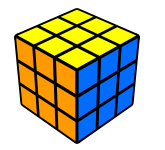
\includegraphics[width=2.5cm]{order.png}
	\caption{order}
	\label{fig:order}
\end{figure}

\begin{figure}[h!]
	\centering
	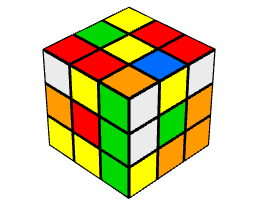
\includegraphics[width=2.5cm]{misorder.png}
	\caption{misorder}
	\label{fig:misorder}
\end{figure}

Solving algorithm 1.

CFOP: we need four steps, the cross, first two layers, orientation of the last layer, permutation of the last layer. first, we set a base sssurface and form a cross on it. second, we notice that the cross divide the first two layers below into four areas. third, we deal with the last layer and makes the surface opposed to our base in the same color. Last, we deal with the third layer and recover it.

Solving algorithm 2.

Roux Method: 6 steps in total. 1. we build a 2x2x2 block. 2. we extend this block into 2x2x3, but we should not destroy the original 2x2x2 part. 3. correct edge orientation. 4. complete two layers. 5. permutate and orient so that the remaining corners are solved. 6. permute the last edge


\item \textbf{Exercise 4.}
1. if we can peove that there does not exist a polynomial algorithm that solve the simple path, we can be mathmeticians. i will only focus on the certificate. Luckily, in this question we only need to prove NP. Let the certificate to be the path P. we can simply use $\bigO (|V|)$ to check if the edges on path is in the graph and if the vertices are repeated. This is polynomial and in P. Thus the problem is in NP. Qed.

2. the certificate would be the factor. with the certificate, we only need to find the gcd of the number and the factor. as we know from ve 475, gcd is done in polynomial time, thus NP. Qed. without this hint, this is equivalent to deciding if it is a prime. Qed.

3. the certificate would be the k specific vertices. For each of them, remove the edges that contains the vertex. After k rounds, we check if the edges are removed clearly. if not, the solution is wrong. this only take time complexity of $\bigO (k\cdot |E|)$ or $\bigO (|V|^2)$, since there are at most $\bigO (|V|^2)$ edges in the graph. this polynomial time complexity means NP. Qed.

\item \textbf{Exercise 5.}
No.

Prime Number Theorem says that the probability of a random integer being smaller than N being prime is close to $1/\log n$.

 Assume we have an n digit number, then under decimal. $\sqrt{10^n}$ is not a polynomial time for size n, it is exponential time. However, we can use smarter polynomial algorithms to cope with PRIME problem, see papers for more detail if you want to be a mathmetician. 

\end{itemize}

%========================================================================
\end{document}
















